\documentclass{article}

\usepackage{graphics}
\usepackage[vcentering]{geometry}

\geometry{papersize={6.9in,2.36in}, top=0.05in, bottom=0in, left=0in, right=0in}

\usepackage{tikz}
\usetikzlibrary{
	arrows,shapes,decorations.pathmorphing,backgrounds,positioning,fit,calc,scopes
}


\tikzset{
	auto,
	compartment/.style={
		rectangle, minimum size=9mm, rounded corners=2mm,
		thick, draw=black!15, top color=white,bottom color=black!30
	},
	%
	bigcompartment/.style={
		rectangle, minimum size=20mm, rounded corners=2mm,
		thick, draw=black!30, top color=white,bottom color=black!20
	},
	%
	point/.style={
		circle, inner sep=2pt, fill=black!5
	},
	%
	mytextbox/.style={
		rectangle, text=black!50, thin, 
		draw=white, top color=white,bottom color=white, fill=white
	}
}


% \definecolor{c1}{RGB}{217, 95, 2}
% \definecolor{c2}{RGB}{117, 112, 179}
% \definecolor{c3}{RGB}{231, 41, 138}
% \definecolor{c4}{RGB}{102, 166, 30}

\definecolor{localc}{RGB}{236, 175, 100}
\definecolor{effc}{RGB}{186, 184, 217}
\definecolor{obsc}{RGB}{243, 148, 197}
\definecolor{intc}{RGB}{153, 209, 89}

\usetikzlibrary{arrows.meta}

\begin{document}

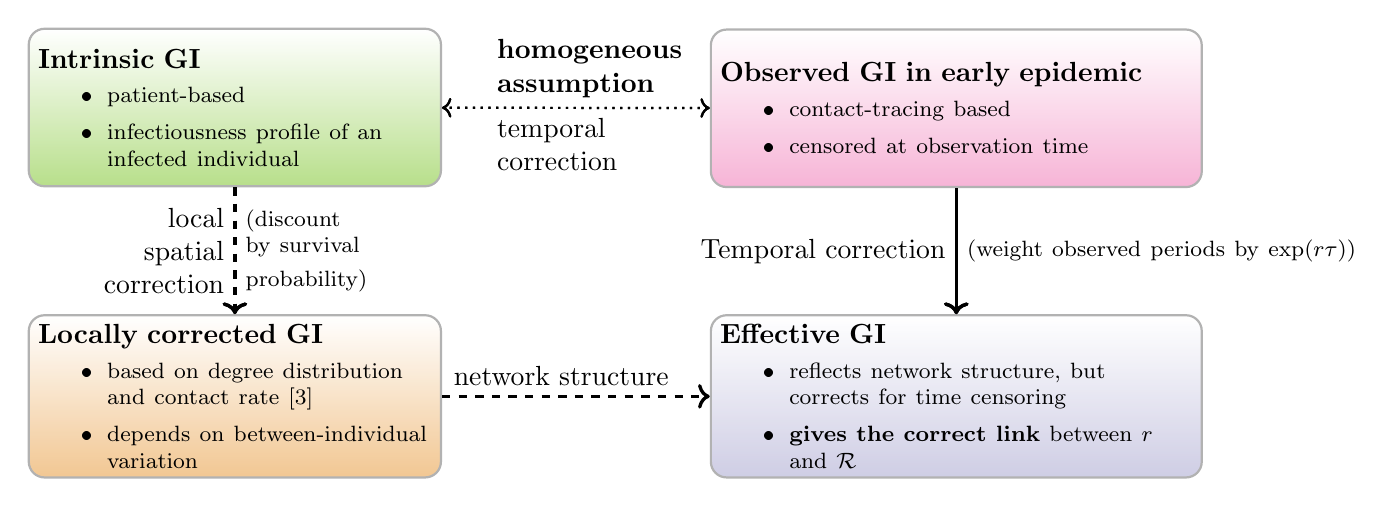
\begin{tikzpicture}
\node(local)[bigcompartment, text width=5cm, bottom color=localc, fill opacity=0.7, text opacity=1]{
    \textbf{Locally corrected GI}
    \footnotesize{
        \begin{itemize}
        	\item based on degree distribution and contact rate [3]
			\item depends on between-individual variation
        \end{itemize}
    }
};

\node(int)[bigcompartment, above=1.61cm of local, text width=5cm, bottom color=intc, fill opacity=0.7, text opacity=1]{
    \textbf{Intrinsic GI}
    \footnotesize{
        \begin{itemize}
        \item patient-based 
		  \item infectiousness profile of an infected individual
        \end{itemize}
    }
};
\draw[->, very thick, dashed] (int) -- node [midway, left, text width=2cm, align=right] {local \\ spatial \\ correction} (local);
\draw[->, very thick, dashed] (int) -- node [midway, right, text width=2cm] {\footnotesize{(discount \\ by survival \\ probability)}} (local);

\node(eff)[bigcompartment, right=3.4cm of local, text width=6cm, bottom color=effc, fill opacity=0.7, text opacity=1]{
    \textbf{Effective GI}
    \footnotesize{
    \begin{itemize}
    \item reflects network structure, but corrects for time censoring
    \item \textbf{gives the correct link} between $r$ and $\mathcal{R}$
    \end{itemize}
    }
};
\node(obs)[bigcompartment, above=1.6cm of eff, text width=6cm, bottom color=obsc, fill opacity=0.7, text opacity=1]{
    \textbf{Observed GI in early epidemic}
    \footnotesize{
    \begin{itemize}
		 \item contact-tracing based
		 \item censored at observation time
    \end{itemize}
    }
};

\draw[->, very thick] (obs) -- node [text width=5cm, midway, left, align=right] {Temporal correction} (eff);
\draw[->, very thick] (obs) -- node [text width=5cm, midway, right] {\footnotesize{(weight observed periods by $\exp(r\tau)$)}} (eff);

\draw[<->, thick, dotted] (obs) -- node [text width=2cm, above]{\textbf{homogeneous\\ assumption}}(int);
\draw[<->, thick, dotted] (obs) -- node [text width=2cm, below]{temporal correction}(int);

\draw[->, very thick, dashed] (local) -- node [text width=3.1cm, above]{network structure}(eff);
% \node(patient)[above left=0cm and 0.2cm of int, rotate=90]{Patient based};
\end{tikzpicture}

\end{document}
